\chapter{System Development}
\label{chp:project}

\section{System Architecture Design}
The design of the system was a crucial part of my internship, consuming approximately 20\% of the total hours dedicated to the project. It was crafted to meet the specific requirements of the business while also taking into account the current context and future needs of the company. UNOX, having collaborated with \ac{AWS} since 2019, leverages innovative \ac{AWS} technologies to maintain a competitive edge. For this project, we were guided by an \ac{AWS} Solution Architect and an Enterprise Account Manager, who played a pivotal role in helping us build a cutting-edge system that adheres to \ac{AWS}'s Well-Architected Framework principles \cite{awswell}, ensuring Operational Excellence, Reliability, Performance Efficiency, Security, Cost Optimization, and Sustainability.

The \ac{AWS} Solution Architect, in particular, provided detailed comparisons of the various \ac{AWS} technologies available, enabling key decision-makers such as myself, the team leader, and the company's CTO to gain a comprehensive understanding of the potential architectures we could build. During the early stages of my internship, we held recurring meetings to explore potential solutions that best aligned with our specific requirements and the nature of UNOX's business operations. These discussions helped us identify the ideal path forward, though the initial solutions inevitably evolved as we encountered and addressed practical challenges during the system's development.

A core aspect of the system design was to ensure a clear separation between the storage layer and the business analytics layer, effectively decoupling data producers (such as operational systems) from data consumers (like reporting and predictive analytics systems). This separation was essential to facilitate data science activities, where a data lake provides a convenient storage layer for experimental data, supporting both the input and output of data analysis and machine learning tasks. The architecture also needed to support autonomous creation and use of data, without the need for coordination between programs or analysts, while at the same time enabling the sharing and re-use of massive datasets through a distributed computational framework.

\subsection{Data Lake vs. Data Warehouse vs. Data Lakehouse}
The initial idea for this project was to implement a data lake, a more innovative and flexible approach compared to traditional data warehouses. While both are used for storing large volumes of data, they serve different purposes and have distinct architectural characteristics.

Traditionally, a \textbf{data warehouse} is optimized for structured data, meaning data is cleaned, organized, and stored in a predefined schema, making it ideal for business reporting and analytics. However, data warehouses typically involve high setup and maintenance costs, and they require significant preprocessing to ensure data consistency before it can be used for analysis. Hence, they suffer from limited flexibility for advanced analytics, including machine learning tasks.

A \textbf{data lake}, on the other hand, offers a more flexible storage solution. It is capable of storing vast amounts of both structured and unstructured data in its raw form, allowing for greater adaptability. This means that data lakes are not bound by rigid schemas and can accommodate data from diverse sources without the need for heavy preprocessing. Data lakes are particularly suitable for data science, machine learning, and exploratory analysis, as they allow analysts and data scientists to directly interact with raw data, creating an environment where experimentation can thrive. A detailed analysis of the differences between data warehouses and data lakes is given in Table \ref{tab:dataw} \cite{nambiar2022overview}.

\begin{table}[h!]
\centering
\begin{tabular}{|p{2.5cm}|p{6.25cm}|p{6.25cm}|}
\hline
\textbf{Parameters}        & \textbf{Data Warehouse}                                      & \textbf{Data Lake}  \\ \hline
\textbf{Data}              & Focuses only on business processes                           & Stores everything   \\ \hline
\textbf{Processing}        & Highly processed data                                        & Mainly unprocessed data                                     \\ \hline
\textbf{Type of Data}      & Mostly in tabular form and structured                        & Can be unstructured, semi-structured, or structured  \\ \hline
\textbf{Task}              & Optimized for data retrieval                                 & Share data stewardship  \\ \hline
\textbf{Agility}           & Less agile, has a fixed configuration                        & Highly agile, can be configured and reconfigured as needed \\ \hline
\textbf{Users}             & Widely used by business professionals and business analysts  & Used by data scientists, data developers, and business analysts  \\ \hline
\textbf{Storage}           & Expensive storage for fast response times                    & Designed for low-cost storage                                       \\ \hline
\textbf{Security}          & Allows better control of the data                            & Offers less control  \\ \hline
\textbf{Schema}            & Schema on writing (predefined schemas)                       & Schema on reading (no predefined schemas)                           \\ \hline
\textbf{Data Processing}   & Time-consuming to introduce new content                      & Helps with fast ingestion of new data                               \\ \hline
\textbf{Data Granularity}  & Data at the summary or aggregated level of detail            & Data at a low level of detail or granularity                        \\ \hline
\textbf{Tools}             & Mostly commercial tools                                      & Can use open-source tools such as Hadoop or MapReduce             \\ \hline
\end{tabular}
\caption{Comparison between Data Warehouse and Data Lake}
\label{tab:dataw}
\end{table}

For this project, the data lake was selected because it enables autonomous data handling, and data producers do not need to coordinate directly with consumers. It also provides a shared storage framework, which facilitates collaboration between teams and allows for the re-use of large datasets without duplication or complex integration.

However, while data lakes excel in flexibility, they can sometimes suffer from challenges related to data governance, data quality, performance, and metadata management. As a result, organizations have adopted a two-tier architecture: storing data in lakes and then moving curated data to warehouses for structured analytics.
The two-tier model (data lakes + data warehouses) introduces new complexities, including reliability and cost issues. Indeed, maintaining consistency between the lake and warehouse is complex and storing data in two places and running \ac{ETL} processes increase costs.

This is where a more modern architecture, the \textbf{Data Lakehouse} \cite{armbrust2021lakehouse}, promoted by Databricks\footnote{\url{https://www.databricks.com/}}, a cloud platform built on Apache Spark that enables unified data analytics, machine learning, and big data processing, comes into play.

The lakehouse architecture combines the best features of both data lakes and data warehouses. It retains the ability of a data lake to store raw and semi-structured data while incorporating some of the data management and performance optimization features of a data warehouse. This hybrid approach allows for real-time analytics and \ac{ACID} transactions on large datasets by adding structured layers of metadata to the raw data.
In fact, the system developed in this project can be interpreted as a data lakehouse. Although it functions primarily as a data lake, we have integrated several layers that provide pre-aggregated tables in Parquet or Iceberg formats, which are directly usable for advanced analysis. These formats not only offer significant performance benefits through better compression and faster query times but also enable \ac{ACID} operations. This structured approach allows us to maximize the system's potential for advanced business intelligence while maintaining the flexibility and scalability inherent in a data lake.

\subsection{The whole system}
\label{sec:wholesystem}

The architecture of the entire system, as illustrated in Figure \ref{fig:wholesystem}, was designed to meet the company’s specific requirements, leveraging cloud technologies to handle large volumes of data while ensuring performance, reliability, and cost-efficiency. The solution automates the process of ingesting, transforming, and analyzing data from various sources, providing a centralized platform for data storage and business intelligence.

\begin{figure}[H]
    \centering
    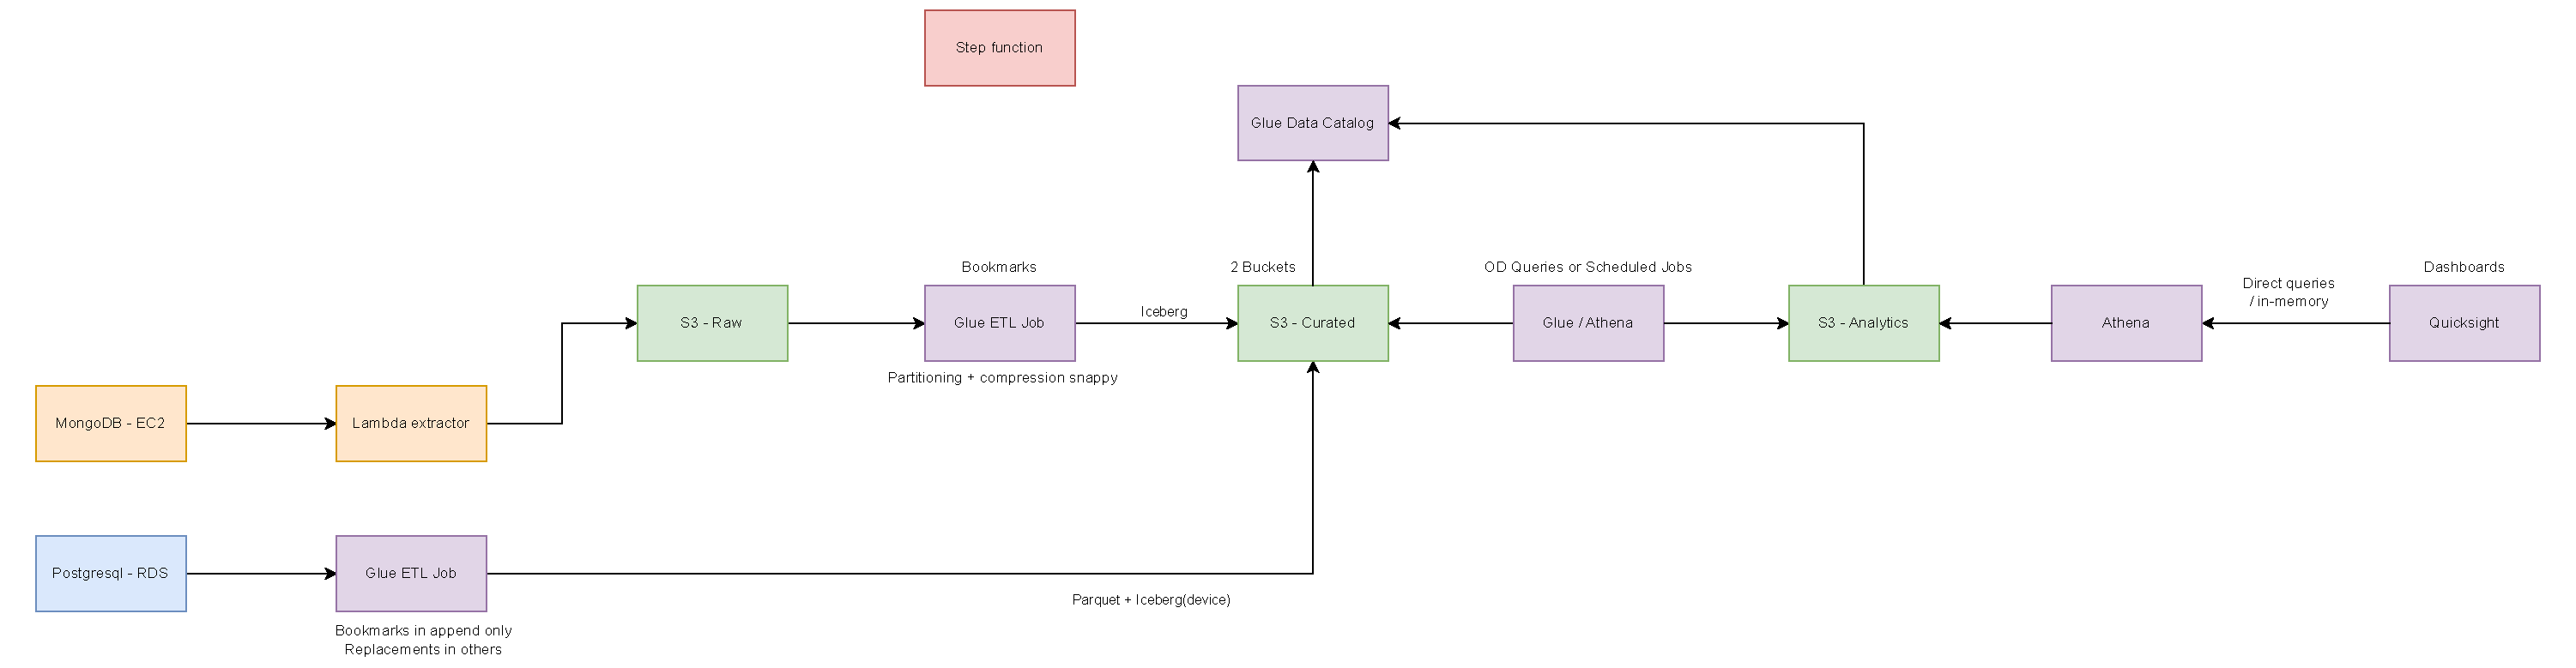
\includegraphics[width=1\textwidth]{res/unox-datalake-v2.pdf}
    \caption{The Whole System}
    \label{fig:wholesystem}
\end{figure}

The system starts with data being collected from two main sources: PostgreSQL for operational data and MongoDB for IoT data generated by the ovens. Each of these data sources follows a custom extraction process. For PostgreSQL, \ac{AWS} Glue is used to execute \ac{ETL} jobs that extract the data, convert it into optimized formats, and load it into Amazon \ac{S3}. For MongoDB, the system uses \ac{AWS} Lambda to manage event-driven data extraction, processing the data and storing it in \ac{S3} in a scalable and efficient way.

Once the data is in \ac{S3}, it is organized into three layers:
\begin{itemize}
    \item \textbf{Raw}: Where the data is stored as extracted, without any transformation.
    \item \textbf{Curated}: Where the data is cleaned, formatted, and partitioned for better query performance.
    \item \textbf{Analytics}: Where the data is pre-aggregated and optimized for specific use cases, such as business reports.
\end{itemize}
The system relies on \ac{AWS} Glue Data Catalog to manage metadata, enabling easy access and query capabilities. For queries, \ac{AWS} Athena is used to allow \ac{SQL} queries directly on the data stored in \ac{S3}, while \ac{AWS} QuickSight provides interactive dashboards and visualizations for business users to explore and analyze the data in real time.

In the following sections, a detailed description of the entire workflow will be provided, including how data ingestion, integration, and cataloguing are performed, as well as how queries and reports are generated. This chapter will also cover how orchestration and scheduling are managed through \ac{AWS} Step Functions, ensuring that each component of the system works seamlessly and in the correct sequence.


\section{Data Sources}

\subsection{PostgreSQL Data}
The Postgres database in this system contains crucial operational data, including various datasets related to Unox ovens and their usage. Managed by \ac{AWS} RDS (as detailed in section \ref{sec:rds}), this instance uses a \texttt{db.t3.xlarge} configuration, providing 4 vCPUs, 16 GB RAM, and 100 GiB of gp2 storage. The database runs PostgreSQL version 12.19, and backups are automatically created every 14 days to ensure data safety.

PostgreSQL hosts several databases, among which the most heavily used is the \texttt{ddc} database. The name \texttt{ddc} refers to the \acf{DDC} platform, an intelligent cooking system that leverages data to optimize and enhance cooking processes. \ac{DDC} offers advanced features for oven owners, enabling them to efficiently monitor and control their devices.

The \texttt{ddc} database comprises 72 tables, with the most critical ones being:
\begin{itemize}
    \item \textbf{Device}: Contains detailed information about all network-connected devices produced by Unox.
    \item \textbf{Company}: Stores information regarding the companies that own Unox ovens.
    \item \textbf{Device group}: Facilitates grouping of devices within a company, allowing management differentiation based on factors such as location, model, or other criteria.
    \item \textbf{Device recipe}: Tracks the current recipe loaded on a device.
\end{itemize}
The relational schema of the main tables is shown in the figure \ref{fig:relschema}. In this diagram, diamonds represent relationship tables, while arrows indicate foreign key relationships pointing to the primary key of the referenced table.
\begin{figure}[H]
    \centering
    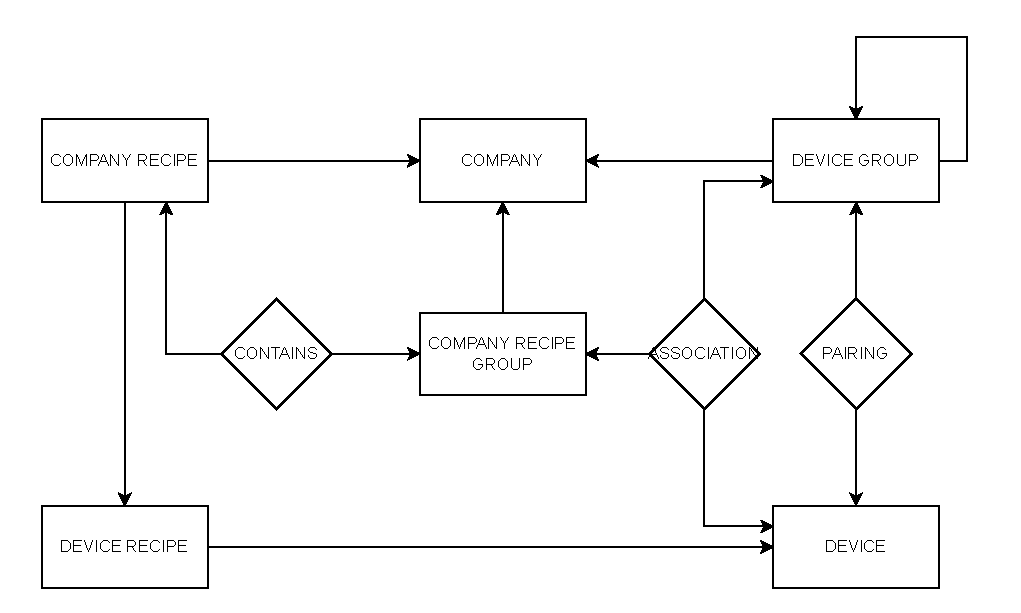
\includegraphics[width=1\textwidth]{res/db-schema.pdf}
    \caption{Main tables relational schema}
    \label{fig:relschema}
\end{figure}
As seen in the diagram, recipes related to a company can also be differentiated based on the device group. This means that recipes can apply at different levels: specific to a device, to a group of devices, or to an entire company. Furthermore, recipes can be created by the community or by Unox itself, stored in the \texttt{community\_recipe} and \texttt{chefunox\_recipe} tables, respectively.

In addition to these, there are other tables related to the primary ones, such as those containing data on the parameters, profiles, or settings of a company or device.

Two more tables, \texttt{device\_recipe\_history} and \texttt{device\_ip\_info\_history}, contain historical data. The former records all recipes created since the installation of a device, while the latter stores the history of IP addresses and associated information for a device. These are the largest tables in terms of storage, with \texttt{device\_recipe\_history} occupying 22 GB and \texttt{device\_ip\_info\_history} storing 5 GB of data.

\subsection{MongoDB Data}
Since \ac{AWS} RDS does not support the MongoDB engine, this database is installed on an \ac{AWS} \ac{EC2} machine. The \ac{EC2} instance used is a \texttt{c5.4xlarge}, with 16 vCPUs and 32 GiB of RAM. The C5 instances are optimized for compute-intensive workloads and offer high performance at a low cost, providing an optimal balance between price and computational power.

Unfortunately, the MongoDB database is deployed on a single replica set and is not configured as a sharded cluster. A replica set consists of a group of MongoDB instances that maintain the same dataset, providing redundancy and high availability. However, without a sharded cluster, the system cannot horizontally scale across multiple nodes, which limits its ability to handle large-scale datasets and high read/write throughput efficiently.

MongoDB organizes data into collections and documents, which can be thought of as equivalent to tables and rows in a relational database, respectively. A document in MongoDB is a flexible, schema-less structure that can be represented as a \ac{JSON}-like object, where there are no constraints on the data types or mandatory fields.

The database contains 20 collections, of which 13 have been deemed useful for analysis and inclusion in the data lake. Table 3.3 describes all the collections, including the approximate number of documents and the storage space they occupy.

\begin{table}[h!]
    \centering
    \begin{tabular}{|l|r|r|r|}
    \hline
    \textbf{Collection} & \multicolumn{1}{l|}{\textbf{Total \# of}} & \multicolumn{1}{l|}{\textbf{Size}} & \multicolumn{1}{l|}{\textbf{Storage Size}} \\ 
                        & \multicolumn{1}{l|}{\textbf{Documents}}   &  &          \\ \hline
    \texttt{alarm}                & 43 M    & 3.7 GiB & 1.9 GiB \\ \hline
    \texttt{end\_of\_prog}        & 240 M   & 60 GiB & 24.7 GiB \\ \hline
    \texttt{end\_of\_prog\_aggregated} & 29 M    & 16.2 GiB & 15.8 GiB \\ \hline
    \texttt{events}               & 1500 M  & 152.6 GiB & 78.2 GiB \\ \hline
    \texttt{evereo\_sess}         & 215 K   & 48.4 MiB & 20 MiB \\ \hline
    \texttt{request}              & 820 K   & 60.7 GiB & 38.8 GiB \\ \hline
    \texttt{sd\_events}           & 75 M    & 11.2 GiB & 5.2 GiB \\ \hline
    \texttt{sd\_haccp}            & 220 M   & 90.3 GiB & 23.6 GiB \\ \hline
    \texttt{sd\_messages}         & 220 M   & 130 GiB & 25.3 GiB \\ \hline
    \texttt{sd\_variables}        & 190 M   & 505 GiB & 156.2 GiB \\ \hline
    \texttt{sdata}                & 170 K   & 80.6 MiB & 29 MiB \\ \hline
    \texttt{variable\_logs}       & 970 M   & 7.3 TiB & 1.8 TiB \\ \hline
    \texttt{working\_minutes\_logs} & 180 K  & 29.3 MiB & 8.6 MiB \\ \hline
    \end{tabular}
    \caption{MongoDB collections used for analysis, with document counts and storage sizes.}
\end{table}

All the collections store time series data, which means that they record sequences of data points indexed in time order. Consequently, each collection includes an \texttt{idDevice} field, indicating which device produced the specific document, and a timestamp field that records when the data was generated. In addition to these, each collection contains specific fields that characterize its data.

As we specified earlier, the data belonging to these collections are generated by the various sensors installed in the devices. When the device is connected to the internet and ready for transmission, the collected data is sent to the back-end, which is responsible for uploading it to the database. The back-end implements a retention mechanism, ensuring reliability in case of database unavailability or upload issues. If a problem occurs, the device is alerted that the data upload was unsuccessful, meaning the device must reattempt the upload once it is ready to transmit again. This mechanism provides robustness, preventing data gaps and duplicates across MongoDB collections. Each device, therefore, uploads data independently, with unpredictable upload intervals.

After successfully uploading the documents to MongoDB, the system updates the \texttt{last\_log\_date} timestamp in the \texttt{device} table of the DDC database. This field reflects the timestamp of the most recent document uploaded for the respective device. Observing this \texttt{last\_log\_date} column, we can confirm that all data with earlier timestamps has been successfully uploaded. However, there may still be additional data recorded by the device that has not yet been uploaded to MongoDB.

It is worth noting that the \texttt{variable\_logs} collection is the largest in terms of data size and will be described in detail in the following section.
\subsubsection{Variable Logs}
The \texttt{variable\_logs} collection represents a time series that captures telemetry data from the ovens. Every 30 seconds, each oven sends data for every available sensor. Each sensor is represented by a variable, and there are sensors that measure various parameters, such as temperature, humidity, fan speed, microwave activity, and other values related to the engine or power supply. For each of these groups, multiple sensors may exist. For example, temperature can be measured in several locations, including the cooking chamber, the core probe, the control board, or the power board. There may also be temperature values such as the one set by the user or the one recommended by algorithms. Additionally, measurements may be sent by accessories connected to the oven.

Each oven can send up to 30-35 measurements every 30 seconds to the back-end, which handles the writing to the database. However, only some of these measurements are actually sent, depending on the oven family, model, and the type of program that is running.

Unfortunately, the document structure in this collection is not very intuitive. Each document represents a 6-hour slot of measurements for a single sensor, divided into 6 one-hour samples, with each sample containing 120 measurements (one every 30 seconds). This format is optimized for the oven’s internal algorithms and is maintained for backward compatibility.

From an analytical perspective, this pattern is somewhat inconvenient. When querying data for specific time periods, a single query returns 720 measurements, and to locate a precise measurement, one must navigate through the nested structure of the \ac{JSON} document.

To address this issue, a view of the collection was previously created, called \texttt{variable\_logs\_clean}, using an aggregation pipeline composed of 7 stages. This view transforms the data structure into a more accessible format by unpacking each document so that there is a single document for each individual measurement, associating it with the specific timestamp of that measurement. Non-existent measurements are excluded from the view, thus preventing the creation of unnecessary documents. This solution results in a significant increase in the number of documents, but each document is much lighter in terms of storage.

For convenience, in the data lake, the view \texttt{variable\_logs\_clean} will be used as the source for oven telemetry data instead of the original collection.

\section{Data Ingestion}
As outlined in the introduction, the data ingestion process differs depending on the two main data sources used in the system: PostgreSQL and MongoDB. These differences arise from the unique requirements of each database and the technologies used to connect and extract data.

For PostgreSQL, AWS Glue establishes a connection using \ac{JDBC}. \ac{JDBC} is a standard API that facilitates communication between a client and a relational database, enabling Glue to execute queries, extract data, and transform it for storage in a structured format like Parquet. This process is crucial for handling structured data efficiently.

In contrast, for MongoDB, the ingestion process involves a direct connection using a MongoDB-specific driver. This type of connection allows the system to interact with MongoDB. Unlike \ac{JDBC}, the driver is tailored for the unique characteristics of MongoDB, allowing for seamless handling of unstructured or semi-structured data.

Due to the need for multiple sequential jobs to export data effectively, it is essential to be able to select specific data subsets for each job. In PostgreSQL, AWS Glue jobs handle this through incremental data ingestion allowed by Bookmarks, while for MongoDB, a different approach was required. To achieve scalability and flexibility in handling the unstructured data from MongoDB, AWS Lambda was chosen as the ingestion tool.

\subsection{PostgreSQL Data}
\subsubsection{Connection to the database}
Before building the actual extraction job for PostgreSQL, it was essential to configure the connection to the database. AWS Glue facilitates the management of connections through a dedicated section where various parameters can be defined. However, prior to configuring this, it was necessary to analyze the company’s networking architecture on AWS.

In AWS, networking is managed through a Virtual Private Cloud (VPC), which is a virtual network dedicated to an AWS account. A VPC can contain multiple subnets, which are smaller segments of the VPC used to organize and isolate resources within different parts of the network. Subnets can be public or private, depending on whether they are associated with an Internet Gateway (IGW) that allows communication with the internet. Security Groups act as virtual firewalls, controlling inbound and outbound traffic for AWS resources. Routing Tables are used to manage the paths that data packets take to reach various destinations, such as other AWS resources or external networks via the Internet Gateway.

In this specific setup, the PostgreSQL RDS (Relational Database Service) instance is distributed across three subnets, all of which belong to the same VPC. These subnets share a single routing table that contains an Internet Gateway, allowing communication with external networks, including the internet.

To configure the connection to the RDS instance, several parameters had to be specified:
\begin{itemize}
    \item \textbf{Database credentials}: This includes the connection type, host, username, password, and port number.
    \item \textbf{Networking details}: The VPC, subnet, and security group had to be defined to ensure that Glue could securely connect to the RDS instance.
\end{itemize}
Once these were set up, it was necessary to create a VPC Endpoint in the routing table. A VPC endpoint enables a private connection between AWS services (in this case, RDS and Glue) without the need to traverse the public internet. In this context, the VPC Endpoint was crucial for allowing Glue to access the RDS instance directly and securely within the VPC. This reduces latency and enhances security by keeping traffic within AWS's private network.

\subsubsection{ETL Job description}
\label{sec:gluejobdesc}
After setting up the connection to the PostgreSQL database, the next step was to create the actual ETL (Extract, Transform, Load) job for data extraction. AWS Glue provides a powerful environment for automating ETL workflows, and each Glue job operates as a script written in either Python or Scala, leveraging Apache Spark as the underlying engine for distributed data processing.

A Glue job typically consists of an ETL script, which can be generated visually or written manually. This script is executed in a serverless environment, meaning there is no need to manage the infrastructure, as Glue handles the allocation of resources dynamically. The ETL script operates using a GlueContext, a specialized context that integrates AWS Glue-specific features into Spark’s ecosystem. GlueContext provides the necessary methods to read from and write to various data sources, like databases, S3 buckets, and data catalogs.

Data in Glue is stored in a structure known as a DynamicFrame, which is similar to Spark’s DataFrame but with added flexibility for semi-structured or schema-less data. A key difference between a DynamicFrame and a DataFrame lies in the level of schema enforcement. While a DataFrame in Spark is strictly tied to a predefined schema, a DynamicFrame is schema-aware but more flexible, allowing it to adapt to evolving data structures. DynamicFrames are especially useful in ETL processes that involve reading from semi-structured sources where data may not adhere to a rigid schema.

As outlined in section \ref{sec:glue}, AWS Glue simplifies the creation of ETL jobs through a fully visual interface. Glue jobs are structured as workflows, which consist of multiple steps that can be executed either sequentially or in parallel. The visual interface allows users to design a flowchart, where each node represents a specific step in the job. These nodes are categorized as Source, Transformation, or Target, depending on the role they play in the ETL process.

For example, in the simplest case of moving a dataset from one location to another, only two nodes are required: a Source node to define the data source and a Target node to specify the destination. Additional parameters such as bookmark usage (to track job progress), execution type, timeout settings, and the database connection are configured globally at the job level. AWS Glue automatically transforms the visual ETL workflow into a Python or Scala script. Therefore, each time the job is executed, it runs the script that was generated based on the visual design. Each node in the flowchart corresponds to a function call, either from Apache Spark or from AWS Glue’s specific libraries.

While visual ETL tools are convenient and intuitive for building basic workflows, they have limitations. They do not always expose all the parameters or advanced options available in the GlueContext or SparkContext. This is particularly restrictive when more granular control is needed, such as fine-tuning the performance of data extraction or transformation steps. For this reason, a custom Python script was written for the PostgreSQL extraction. This approach allowed for full utilization of Glue's and Spark's capabilities, ensuring optimal performance and flexibility. Using a custom script also allowed for more advanced data filtering, error handling, and optimization techniques.


\subsubsection{Glue Bookmarking in JDBC Sources}

In the context of AWS Glue, \textit{bookmarks} serve as a mechanism to track the progress of a job by saving the last processed primary key. Specifically, for JDBC sources, the bookmark stores the value of the last primary key that was successfully processed during the job execution. This information is stored in an internal JSON file in Glue's storage system. When the job is run again, it checks whether a bookmark is present for each table. If a bookmark exists, the job filters the data by selecting only those rows where the primary key is greater than the one saved in the bookmark, ensuring that only new rows are imported.

However, this functionality presents certain limitations. If a row in the source table is updated, but its primary key remains unchanged, the updated row will not be selected during the next job execution, leading to outdated data in the data lake. On the other hand, if the primary key changes during the update, the updated row is imported into the data lake, but the old version of the row remains, resulting in duplicated data. Consequently, the use of bookmarks is only advantageous in cases where the source table is append-only, meaning no updates or deletions are performed.

Given these constraints, specific solutions have been proposed depending on the behavior of the tables in the company's \texttt{ddc} database:
\begin{itemize}
    \item For tables that only undergo append operations, the use of bookmarks is feasible, allowing the job to load only the newly inserted rows. This helps optimize the data ingestion process.
    \item For tables that undergo upserts (i.e., updates or inserts), a more efficient solution is to replace the entire table during each job execution. This involves deleting the previous version of the table in the data lake and replacing it with the updated version from the source. Since the total memory occupied by these tables is less than 300 MB, this approach is manageable from a performance and cost perspective.
    \item A special case is the \texttt{device\_recipe} table, which deletes a row and reinserts it with a new primary key whenever an update occurs. Given the size of this table (approximately 1 GB), the most effective solution is to replace the entire table in the data lake after each job execution to ensure data consistency.
    \item The \texttt{device} table also behaves similarly to \texttt{device\_recipe}, but with an additional requirement for \textit{Time Travel}. Time Travel is a feature that would be useful in this context to retain historical data, such as older firmware versions installed on the devices or previous IP addresses. In this case, the use of Apache Iceberg is proposed as a solution. Iceberg is a table format designed for large-scale datasets, providing capabilities such as schema evolution, partitioning, and Time Travel. During each job execution, the entire \texttt{device} table (around 70 MB) would be loaded, and, if the table is already present in the data lake, a \texttt{MERGE INTO} operation would be performed.
\end{itemize}
The \texttt{MERGE INTO} operation in Iceberg works by combining data from two tables based on a matching condition. Specifically, it checks for rows that already exist in the target table and updates them with the new data from the source. If a row in the source table does not have a matching row in the target table, it is inserted as a new row. This process ensures that both the updated and new rows are correctly handled without creating duplicates.

While performing a \texttt{MERGE} between two tables that are nearly identical (with only a few updated rows) is not the most efficient operation, a proposed optimization is to load only the rows with a recent \texttt{updated\_at} timestamp. This column, which indicates the time at which a row was last updated, can be used to filter rows that have been updated within a certain time frame. For example, a query like \texttt{SELECT * FROM device WHERE updated\_at >= NOW() - INTERVAL '2 DAYS'} would select only the rows that have been updated in the last two days, reducing the amount of data that needs to be processed during the \texttt{MERGE INTO} operation.

However, due to inconsistencies in the \texttt{updated\_at} column, it was ultimately decided to perform the \texttt{MERGE} with the entire table as the source, ensuring that no updates are missed.

Before diving into the specifics of the implemented script, it is worth mentioning that the entire solution could have been replaced by a \ac{CDC} system, for example using AWS \ac{DMS}. AWS DMS allows for continuous replication of data changes from a source database to a target location, capturing inserts, updates, and deletes in real-time. By leveraging CDC, it would be possible to automatically detect and replicate any change in the PostgreSQL database to the data lake, eliminating the need for periodic full-table exports. However, this solution was discarded due to the high costs associated with its constant execution, as DMS would require a continuous running process to capture all changes.

\subsubsection{Glue Script}

The exporting code is divided into three distinct phases, each processing a subset of tables sequentially based on their characteristics and behavior. Below is a detailed explanation of each part of the script.

\paragraph{First Phase: Processing Upsert Tables}

The first part of the script processes tables that can undergo upsert operations (update or insert). The array \texttt{tableNames} contains the list of tables to be processed, which was generated by querying the \texttt{information\_schema.tables}, a system table that holds metadata about all tables in the database. From this set, append-only tables were excluded.

The following code snippet illustrates how each table is processed:

\begin{lstlisting}[language=Python, caption=First phase Postgres extraction]
for tableName in tableNames:
    logger.info("TABLE: " + str(tableName))
    table = glueContext.create_dynamic_frame.from_options(
        connection_type = "postgresql",
        connection_options = {
            "useConnectionProperties": "true",
            "dbtable": tableName,
            "connectionName": "Postgresql connection production",
        }
    )
    
    objects_to_delete = s3.list_objects_v2(Bucket="datalake-postgres", Prefix=tableName+"/")
    if 'Contents' in objects_to_delete:
        delete_keys = {'Objects': [{'Key': obj['Key']} for obj in objects_to_delete['Contents']]}
        s3.delete_objects(Bucket="datalake-postgres", Delete=delete_keys)

    out = glueContext.getSink(path="s3://datalake-postgres/"+tableName+"/", connection_type="s3", updateBehavior="UPDATE_IN_DATABASE", partitionKeys=[], enableUpdateCatalog=True, transformation_ctx="write_"+tableName)
    out.setCatalogInfo(catalogDatabase="postgres", catalogTableName=tableName)
    out.setFormat("glueparquet", compression="snappy")
    out.writeFrame(table)
\end{lstlisting}

The \texttt{glueContext.create\_dynamic\_frame.from\_options()} function reads the PostgreSQL table and converts it into a \texttt{DynamicFrame}, which can then be manipulated and written to other destinations. Since these tables undergo upserts, it is necessary to delete the existing tables in Amazon S3 to replace them with the updated version. This is done using the \texttt{list\_objects\_v2()} and \texttt{delete\_objects()} methods from the \texttt{boto3} client. \texttt{boto3} is the AWS SDK for Python, which allows to interact with AWS services, such as S3.

After clearing the existing data, the updated \texttt{DynamicFrame} is written back to S3 in Parquet format using \texttt{glueContext.writeFrame()}. The data is automatically added to the AWS Glue Data Catalog, making it available for further querying and processing. The use of the \texttt{Snappy} compression format ensures efficient storage.

\paragraph{Second Phase: Processing Append-Only Tables}

The second phase processes tables that are append-only, meaning that new rows are only added, and no updates or deletions occur. This phase is similar to the first one, but with a few key differences. First, in this case, the use of bookmarks is enabled, allowing the job to only load new rows since the last execution. This is achieved by configuring the \texttt{transformation\_ctx} parameter, which ensures the bookmark functionality tracks the last processed row and continues from that point during the next run.

Furthermore, since some of these append-only tables (as discussed in section \ref{sec:database_tables}) contain a large amount of data, it was necessary to optimize the read operations. This was done by using the \texttt{hashfield} and \texttt{hashpartition} parameters. These parameters enable partitioning of the data based on a hash of the specified field, which allows for parallel processing, improving the performance of reading large tables. The \texttt{hashfield} determines the column used for hashing, and \texttt{hashpartition} defines how many partitions the data should be split into for parallel execution.

\paragraph{Third Phase: Processing the Device Table with Time Travel}

The third phase of the script processes the \texttt{device} table, which involves upsert operations and requires \textit{Time Travel}. To enable Time Travel, the table is stored in Apache Iceberg format, which supports versioning and allows efficient retrieval of data from different historical snapshots.

Below is the snippet that handles the \texttt{MERGE INTO} operation for the \texttt{device} table:

\begin{lstlisting}[language=SQL, caption=MERGE INTO for Postgres extraction]
MERGE INTO glue_catalog.postgres.device t
USING merge_source s
ON t.id = s.id
WHEN MATCHED AND (t.id_firmware <> s.id_firmware OR t.board_serial <> s.board_serial OR t.id_board_model <> s.id_board_model OR t.last_ip <> s.last_ip OR t.city <> s.city OR t.connection_kind <> s.connection_kind OR t.bridge_firm <> s.bridge_firm OR t.cloud_pin <> s.cloud_pin OR t.mirror <> s.mirror) THEN
    UPDATE SET *
WHEN NOT MATCHED THEN
    INSERT *
\end{lstlisting}

The \texttt{MERGE INTO} operation compares the rows from the source table (designated as \texttt{s}) with the target table (designated as \texttt{t}). If a matching row is found (based on the \texttt{id}), and any of the key fields (such as firmware, board serial, or IP address) has changed, the row in the target table is updated. If no matching row is found, the new row from the source table is inserted into the target. This ensures that the table in S3 remains synchronized with the PostgreSQL source, while also maintaining historical data for Time Travel purposes.

\subsection{MongoDB Data}
For the IoT data stored in MongoDB, a completely different approach was adopted. AWS Glue does not support bookmarks for connections other than JDBC and S3, which ruled out the possibility of using Glue’s native bookmarking functionality. Additionally, several challenges made it impractical to create a custom bookmark system in Glue. One such limitation is that the functions provided by the Glue context do not support \textit{pushdown predicates}, which are conditions applied at the data source level to limit the data returned. Without pushdown predicate support, every time a collection is read, it must be fully imported and then filtered afterward. Importing several terabytes of data with each job execution is clearly unfeasible.

In principle, \texttt{pyspark} provides a \texttt{read()} function that allows passing an aggregation pipeline as a parameter. An aggregation pipeline is a MongoDB framework that processes data through multiple stages, each applying specific transformations or filtering conditions to the dataset. While this approach would work for ongoing operational tasks, during the initial ingestion phase, it would still be highly inefficient due to the large data volume. Handling this with multiple aggregation pipelines, each importing a subset of data, would require sequential execution in Glue, as asynchronous operations are not supported in this environment, significantly increasing execution time.

Given these constraints, it was decided to use AWS Lambda functions, which offer scalability based on workload, parallel execution, and support for asynchronous queries. AWS Lambda is a serverless compute service that runs code in response to events, automatically managing the infrastructure required to execute the code. A notable limitation of Lambda is its maximum execution duration of 15 minutes, which needs to be considered when handling large-scale data processing tasks.

To deploy the Lambda functions, the \texttt{Serverless Framework} was used. This framework enables simplified management of serverless applications by automating the setup, deployment, and scaling of resources, without needing to manually provision or manage servers. The functions were written in Node.js with TypeScript, chosen for its robust asynchronous code handling capabilities and strong type-checking, which enhances code reliability and maintainability.

Two \acp{ORM} were utilized. For PostgreSQL, \texttt{Prisma} was selected to handle bookmarking data, as it allows seamless connections to multiple databases in the same environment. Prisma simplifies data access by generating a type-safe client, which improves both the efficiency and reliability of database interactions. For MongoDB, the original MongoDB driver developed for Node.js was used, offering direct and optimized support for MongoDB’s functionalities and data handling requirements.

To interact with AWS services, the JavaScript \texttt{\ac{SDK} v3} was utilized. AWS \ac{SDK} v3 is the latest version of the Software Development Kit provided by Amazon, specifically designed to facilitate interaction with AWS services. It offers modular packages, each dedicated to a specific service, allowing developers to import only the required functionalities. This approach optimizes application performance by reducing the overall bundle size, which is especially beneficial for serverless environments where minimizing execution time and memory usage is crucial.

The architecture for the Lambda functions consists of two TypeScript-based functions: \textit{master} and \textit{worker}. To initiate the data extraction process, the \textit{master} Lambda function is invoked. This function is responsible for identifying which devices have sent data since the previous job execution and for invoking multiple \textit{worker} Lambdas accordingly. The \textit{worker} Lambdas then handle the export of new data for the identified devices, allowing the system to bypass the 15-minute execution timeout limitation by distributing the workload across multiple functions. Each \textit{worker} Lambda imports data from a single collection and processes a subset of devices. Figure \ref{fig:lamschema} illustrates the architecture of the Lambda-based solution used for the data ingestion process.
\begin{figure}[H]
    \centering
    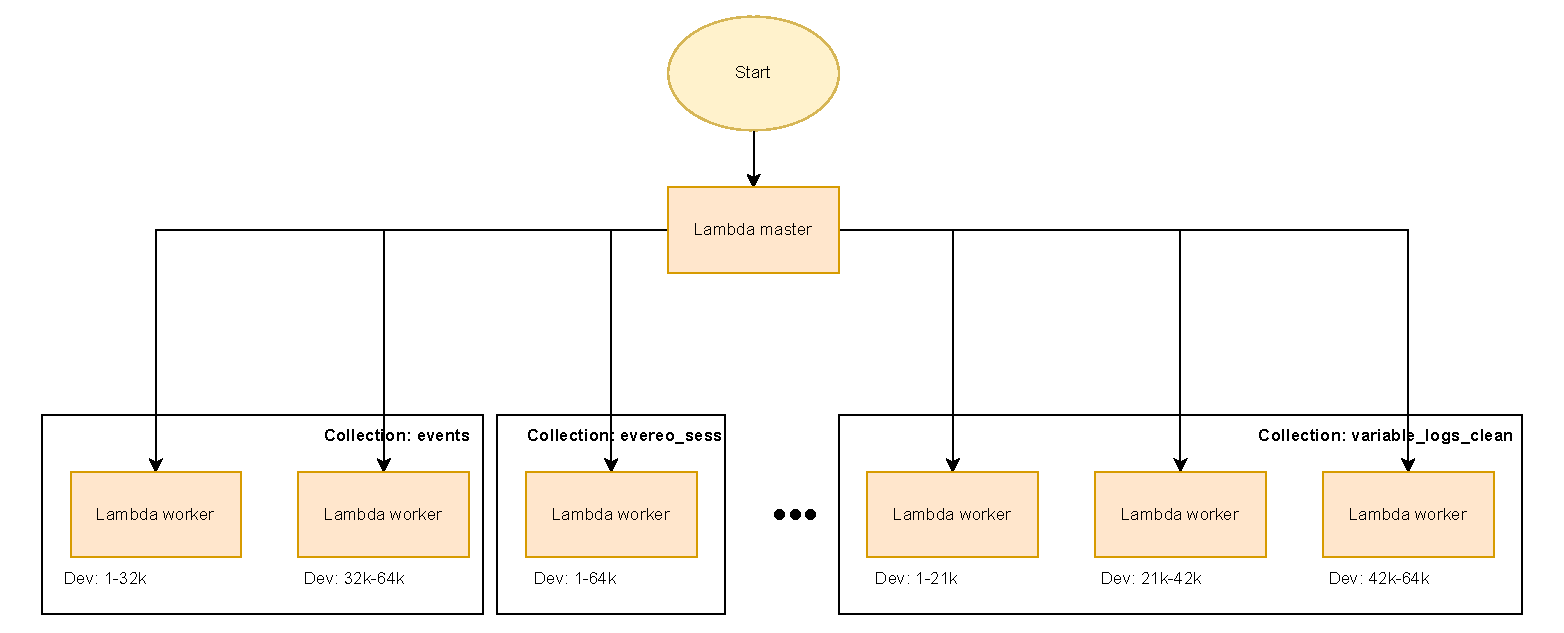
\includegraphics[width=1\textwidth]{res/lambda-schema.pdf}
    \caption{Lambdas architecture}
    \label{fig:lamschema}
\end{figure}

To implement custom bookmarking, a dedicated support database was created in an AWS RDS instance to avoid overloading the production database. This support database includes a table named \texttt{lastts}, designed to track data ingestion progress. The \texttt{lastts} table contains three columns: \texttt{idDevice}, which identifies each specific device, \texttt{collection}, indicating the dataset collection, and \texttt{lastts}, a timestamp indicating the latest ingestion point for the device. Together, \texttt{idDevice} and \texttt{collection} form the primary key, ensuring uniqueness for each device and collection combination.

In addition, the support database includes a table named \texttt{metrics} for tracking processing metrics. Each time a worker completes processing a list of devices, it logs a new entry in the \texttt{metrics} table with details such as: \texttt{First device processed}, \texttt{Last device processed}, \texttt{Devices to query}, \texttt{Documents uploaded}, \texttt{Worker computation time}, \texttt{Total runned queries}, \texttt{Devices processed}, \texttt{Collection}, and \texttt{Number of errors}. These metrics provide valuable insights into job performance, allowing for monitoring and optimization of the data ingestion pipeline.

\subsubsection{Master Function}

The \textit{master function} begins by querying all devices in the \texttt{device} table to obtain their \texttt{last\_log\_date} timestamps. These timestamps represent the latest data logged by each device, which is essential for determining if any new data needs to be processed. For each collection in the system, the function retrieves the \texttt{lastts} timestamp for each device from the \texttt{lastts} table. This \texttt{lastts} timestamp indicates the most recent data ingestion point for that collection. If a device’s \texttt{lastts} does not exist, or if its \texttt{last\_log\_date} is greater than its \texttt{lastts}, the device is added to an array called \texttt{devicesToQuery}, marking it as ready for further processing.

Once the \texttt{devicesToQuery} array is populated for each collection, the function organizes these devices into batches for parallel processing. The batching is controlled by \texttt{workerSize}, which is calculated based on the total number of devices and the preset number of workers specified in \texttt{workersPerCollection}. This object defines the desired number of workers per collection, with collections containing a higher volume of documents assigned a greater number of workers to manage the load more effectively. Alternatively, there is a \texttt{splitMode} option, which specifies a target number of devices per worker, dynamically adjusting the number of invoked workers based on the number of devices identified for processing.

The code snippet below demonstrates the batching and invocation of workers:
    \begin{lstlisting}[language=Python, caption=Device batching]
const workerSize = Math.ceil(devicesToQuery.length / workersPerCollection[operationalMode][collection])
for (let i = 0; i < devicesToQuery.length; i += workerSize)
    invocations.push(invokeWorkerWithTimeout(devicesToQuery.slice(i, i + workerSize), collection))
\end{lstlisting}

The master function manages all worker invocations using \texttt{Promise.allSettled(invocations)}, which executes all promises concurrently and returns an array of results, one for each promise. Each result indicates whether the corresponding promise was fulfilled or rejected. This approach ensures that all worker executions complete, regardless of individual failures, without interrupting the entire process.

The following functions handle each worker invocation:

\begin{lstlisting}[language=Python, caption=\texttt{invokeWorkerWithTimeout} and \texttt{invokeWorker} functions]
async function invokeWorkerWithTimeout(dev: number[], collection: string) {
  const timeoutPromise = new Promise<never>((_, reject) =>
    setTimeout(
      () => reject(new Error(`Timeout for worker ${collection}${dev[0]}`)),
      WORKERS_TIMEOUT,
    ),
  );

  return Promise.race([invokeWorker(dev, collection), timeoutPromise]);
}

async function invokeWorker(dev: number[], collection: string) {
  const params = {
    FunctionName: `datalake-mongo-extractor-${process.env.NODE_ENV}-worker`,
    Payload: JSON.stringify({
      body: {
        devices: JSON.stringify(dev),
        collection: collection,
      },
    }),
  };

  const command = new InvokeCommand(params);
  const response = await lambdaClient.send(command);

  // Handle worker Lambda response
  if (response.StatusCode !== 200) {
    throw new Error(`Invocation failed for a worker`);
  }

  const payload = JSON.parse(new TextDecoder('utf-8').decode(response.Payload));

  if (payload.errorMessage) {
    throw new Error(
      `${payload.errors} error(s) in worker ${payload.id} (${payload.log_stream_name})`,
    );
  }

  return payload;
}
\end{lstlisting}

The \texttt{invokeWorker} function constructs and sends the invocation command for each worker Lambda. If the response \texttt{StatusCode} is not \texttt{200}, an error is thrown, indicating that the invocation failed. Additionally, if there are specific errors reported in the worker's payload, these are also logged as errors.

In this process, three primary types of errors may occur. Each is handled independently by logging the error to avoid affecting other workers or the master function:
\begin{itemize}
    \item \textbf{Worker invocation failure}: If \texttt{InvokeCommand} returns a \texttt{StatusCode} other than \texttt{200}, the invocation did not succeed.
    \item \textbf{Error within the worker}: If the worker encounters any issue, the master function receives a payload containing the number of errors that occurred. Full error details are logged within each individual worker, accessible via AWS CloudWatch.
    \item \textbf{Worker timeout}: If a worker does not complete within 15 minutes, the issue is managed by \texttt{Promise.race()} to which two promises are passed: the actual worker invocation (\texttt{invokeWorker}) and a timeout promise. If the worker exceeds the predefined \texttt{WORKERS\_TIMEOUT} duration, the timeout promise rejects, ensuring the master function is aware that the worker did not complete within the expected time.
\end{itemize}

In this setup, all master and worker logs are available in AWS CloudWatch, enabling easy access to error details and execution summaries. \texttt{CloudWatch} is an AWS tool for monitoring and managing log data from AWS services. 

Once all worker responses are received, the master function logs summary statistics for each collection. This includes progress as a percentage of documents uploaded relative to the total documents in each collection. The uploaded document count is calculated by summing the values in the \texttt{docs\_uploaded} field within the \texttt{metrics} table for a specific collection in the support database. The total document count is estimated using the MongoDB driver's \texttt{estimatedDocumentCount()} function.

Since \texttt{variable\_logs\_clean} is a view and does not support direct document counting, progress is calculated based on the percentage of devices processed relative to the total number of devices. The following function, \texttt{countTotalKeys}, counts the already processed devices:

\begin{lstlisting}[language=Python, caption=\texttt{countTotalKeys} function]
async function countTotalKeys() {
  let totalKeyCount = 0;
  let continuationToken;
  let isTruncated = true;

  while (isTruncated) {
    const params: ListObjectsV2CommandInput = {
      Bucket: AWS_CONFIG.TARGET_BUCKET,
      Prefix: 'variable_logs_clean/',
      Delimiter: '/',
      ContinuationToken: continuationToken,
    };

    const data = await s3Client.send(new ListObjectsV2Command(params));

    // Sum KeyCount from the current response
    totalKeyCount += data.KeyCount ?? 0;

    // Handle pagination
    continuationToken = data.NextContinuationToken;
    isTruncated = data.IsTruncated ?? false;
  }

  return totalKeyCount;
}
\end{lstlisting}

This function iterates through paginated S3 results to count the total keys, providing an approximate measure of processed devices. This estimation is more approximate than document counting and is mainly useful for bulk loads.

Finally, the master function returns a JSON response summarizing the number of successfully executed workers and overall progress, completing the orchestration for data processing and upload.

\subsubsection{Worker function}

As previously discussed, the master function invokes each worker function with two parameters: the \texttt{collection} to process and a list of \texttt{devices}. The worker function begins by adding all devices to an \textit{async queue} with a concurrency level of 5, meaning that up to five tasks can execute concurrently. An \textit{async queue} allows tasks to be processed asynchronously, enabling the execution of multiple tasks in parallel. However, it should be noted that, due to Node.js's single-threaded nature, this parallelism is achieved via asynchronous handling rather than true parallel threads.

Each task in the queue processes a single device, querying and loading its data into the data lake in manageable portions. Given the high volume of data, it is necessary to retrieve records in smaller segments. Starting from the earliest available data in 2015, the function performs sequential queries, each covering a 60-day period, until it reaches the device's \texttt{last\_log\_date}. Due to AWS Lambda's 15-minute maximum execution time, all queries must complete within 10 minutes, leaving a 5-minute buffer to finalize the last query without risking timeout.

Each execution task in the queue involves a \texttt{while} loop, iterating as long as the total runtime is under 10 minutes. In each iteration, the loop defines the query period’s boundaries: \texttt{from} and \texttt{to}. The \texttt{from} value is set to the device’s \texttt{lastts} if available; otherwise, it defaults to October 2015 (the beginning of MongoDB data storage). The \texttt{to} value is determined as the minimum between \texttt{from + 60 days} and \texttt{last\_log\_date}. If \texttt{from} is greater than or equal to \texttt{to}, the loop ends, indicating all data has been imported for that device.

\textbf{Query Construction} \\
Once the time boundaries are defined, the worker constructs a MongoDB query tailored to the specific \texttt{collection}. Since each collection has its own structure and timestamp field names, a custom query format is created for each one. For instance, in the \texttt{variable\_logs\_clean} collection, the query is structured as follows:

\begin{lstlisting}[language=Python,caption=]
variable_logs_clean: (device, from, to) => ({
    idDevice: device,
    day: {
      $gte: new Date(from.getTime() - (from.getTime() % 21600000)),
      $lte: new Date(to.getTime() - (to.getTime() % 21600000)),
    },
    time: { $gt: from, $lte: to },
})
\end{lstlisting}

This query filters by \texttt{idDevice}, with \texttt{from} and \texttt{to} as the start and end times, respectively. The timestamp fields are aligned to the nearest 6-hour interval to match the structure of \texttt{variable\_logs\_clean} documents.

The MongoDB query then runs, with results stored in \texttt{queryResult}. After obtaining the data, it undergoes two main aggregation steps to ensure consistency and format the records properly:

\begin{itemize}
    \item \textbf{Common aggregation}: Applied to all collections, this step moves non-standard fields (those not defined in the Parquet schema for that collection) into a \texttt{payload} field. This standardizes each document by consolidating unusual fields.
    \item \textbf{Variable\_logs\_clean aggregation}: Specific to the \texttt{variable\_logs\_clean} collection, this aggregation combines all measurements with the same timestamp from a single device into one document.
\end{itemize}

\textbf{Data Loading to the Data Lake} \\
Once the documents are ready for data lake ingestion, the worker function performs three crucial steps: updating the \texttt{lastts}, converting JSON documents to Parquet format, and uploading the data to an S3 bucket. It is essential that these three operations are executed robustly, meaning that if any one of them fails, the other steps should not complete. To ensure this robustness, these operations are encapsulated within a transaction managed by Prisma.

In Prisma, \textit{interactive transactions} provide a way to bundle multiple database operations into a single logical unit. Within an interactive transaction, either all operations are successfully completed and committed, or if any operation fails, the transaction is rolled back, undoing any changes made during the transaction. In this context, if either the conversion to Parquet or the upload to S3 fails, the transaction is not committed, effectively rolling back the \texttt{lastts} update. Consequently, the next execution will attempt to re-import the same data. Additionally, if a transaction-level error occurs, the worker ensures any partially uploaded files are removed, maintaining data consistency.

For the conversion of JSON documents to Parquet format, the \texttt{parquetjs} library was utilized. \texttt{parquetjs} allows for efficient transformation of JSON data into Parquet format, a columnar storage format optimized for high-performance querying. The library supports schema definitions, so each collection's schema is specified, ensuring consistent data structure in the output files. Furthermore, both the conversion and upload processes are performed using \textit{streaming}, allowing the function to handle large data volumes without overwhelming memory.

Streaming in Node.js enables data to be processed in chunks, where each data chunk flows continuously from one stage of the pipeline to the next without waiting for the entire dataset. In this implementation, the streaming pipeline begins with a \texttt{Readable} stream that reads data from \texttt{documentsAggregated}, applies the Parquet transformation, and finally streams the transformed data to the S3 destination. Here is the code that accomplishes this:

\begin{lstlisting}[language=Python]
const destination = new PassThrough();
const reader = Readable.from(documentsAggregated);
const pt = new ParquetTransformer(parquetSchemas[params.body.collection]);

await new Promise<void>((resolve, reject) => {
  pipeline(reader, pt, destination).catch((err) => reject(err));

  const upload = new Upload({
    client: s3Client,
    params: {
      Bucket: AWS_CONFIG.TARGET_BUCKET,
      Key: `${params.body.collection}/${device}/${from.getTime()}.parquet`,
      Body: destination,
      ContentType: 'application/parquet',
    },
  });
  upload
    .done()
    .then((res) => resolve())
    .catch((err) => reject(err));
});
\end{lstlisting}

In this code:
\begin{itemize}
    \item \texttt{destination} is a \texttt{PassThrough} stream that serves as the final output in the pipeline.
    \item \texttt{Readable.from(documentsAggregated)} creates a readable stream from the JSON documents, allowing them to be processed sequentially.
    \item \texttt{ParquetTransformer} applies the Parquet schema transformation, converting the JSON data into Parquet format in real-time.
    \item \texttt{pipeline()} connects the readable stream, Parquet transformation, and \texttt{destination} stream in a sequence, with errors caught and handled via \texttt{reject}.
\end{itemize}
The transformed data is then uploaded to S3 using the \texttt{Upload} function, which reads from \texttt{destination} and streams data directly to the S3 bucket, saving memory and speeding up the process.

Once the queue is empty, either due to reaching the time limit or because all devices have been processed, a new entry is added to the \texttt{metrics} table in the support database. This entry records various metrics measured during execution, such as the number of processed devices, total queries executed, and uploaded document count. These metrics are also logged to AWS CloudWatch, where they can be monitored for performance analysis and troubleshooting.

Finally, the worker function returns a response to the master function, including the \texttt{statusCode}, the unique Lambda identifier, and any error counts detected during execution.

\section{Data Integration}
As described earlier, the extracted data is directly stored in two different S3 buckets. AWS S3 is an object storage service that organizes data within containers called \textit{buckets}, each capable of storing virtually unlimited objects. A bucket does not function as a typical directory; rather, each file within S3 is identified by a unique \textit{key}, which may include prefixes resembling folder structures. In this system, PostgreSQL data is stored in a bucket named \texttt{datalake-postgres}, where each table is assigned a distinct prefix corresponding to its table name. MongoDB data, on the other hand, is stored in a bucket named \texttt{datalake-mongodb}, organized with prefixes based on collection names and device IDs.

As introduced in Section \ref{sec:wholesystem}, the data lake structure is composed of three layers: \textit{raw}, \textit{curated}, and \textit{analytics}. For PostgreSQL data, it was decided to combine the raw and curated layers, as data can be cleansed during extraction through the Glue ETL job. Maintaining an additional extraction job and S3 bucket for raw data was deemed unnecessary, given that PostgreSQL tables are relatively lightweight and do not justify the complexity of a separate raw layer.

For MongoDB, however, an ETL job is required to transform data from the raw layer to the curated layer. The structure of this job is similar to that described in Section~\ref{sec:gluejobdesc}, with each collection processed sequentially. It comprises a source node (reading from the raw layer), a transformation node, and a target node (writing to the curated layer). For this transformation, Glue bookmarks are employed to track progress when reading from S3. Unlike JDBC bookmarks, which record the last processed primary key, S3 bookmarks store the last modified timestamp of the files read.

Currently, this ETL job performs four key functions:
\begin{enumerate}
    \item conversion from Parquet format to Iceberg,
    \item Snappy compression,
    \item partitioning,
    \item and deduplication of the \texttt{alarm} collection.
\end{enumerate}
Transforming MongoDB tables to Iceberg format is beneficial primarily for two reasons: Iceberg enables optimized table storage and enhances partitioning capabilities. Table optimizations are covered in detail in Section~\ref{section:}, as these are applied directly within the data catalog. Iceberg’s hidden partitioning also facilitates effective partitioning based on metadata for \texttt{timestamp} columns, as well as customizable partitioning by year, month, or day.

Partitioning of collections was implemented to improve query performance by reducing the scope of data scanned. Specifically, all collections are partitioned by \texttt{idDevice}, and larger collections are additionally partitioned by year. By leveraging Iceberg’s hidden partitioning, data can be partitioned based on timestamps down to the year, month, or day level. To determine the optimal time granularity for partitioning, several tests were conducted (see Section~\ref{section:}), as daily partitioning is not always ideal. While partitioning by day minimizes the amount of data scanned for short-term queries, it significantly increases I/O operations for long-term queries. This results in multiple small files for daily partitions, whereas a monthly partition would only require a single file and a single I/O access. 

In the context of company data, the daily volume for each device and collection does not justify creating a separate file. Additionally, most queries target extended time periods, so partitioning by year was chosen to minimize I/O overhead, thus improving response latency. The downside of this choice is a potential increase in scanned data for certain queries, which may elevate query costs (particularly when using AWS Athena, where costs are based on scanned data size).

\textbf{Deduplication of \texttt{alarm} documents} \\
Deduplication of documents in the \texttt{alarm} collection is necessary because \texttt{alarm} is the only collection in the data lake that may undergo updates. Each document in \texttt{alarm} includes fields such as \texttt{id} (document identifier), \texttt{idDevice} (device identifier), \texttt{code} (alarm code), \texttt{activeTS} (alarm activation timestamp), \texttt{resetTS} (alarm reset timestamp), among others. Here, \texttt{resetTS} is always greater than or equal to \texttt{activeTS}, but a document may initially lack a \texttt{resetTS} if the alarm is active when recorded in the database. The document is subsequently updated with a \texttt{resetTS} once the alarm is deactivated. Consequently, documents are added to the data lake if either \texttt{activeTS} or \texttt{resetTS} is greater than the \texttt{lastts}. Depending on the status of these timestamps during data ingestion, three scenarios can arise:

\begin{itemize}
    \item \texttt{activeTS} and \texttt{resetTS} are both greater than \texttt{lastts}: No deduplication is required.
    \item \texttt{activeTS} is greater than \texttt{lastts} and \texttt{resetTS} does not exist: The document will be re-imported when \texttt{resetTS} becomes available, requiring deduplication.
    \item \texttt{activeTS} is less than \texttt{lastts} and \texttt{resetTS} is greater than \texttt{lastts}: The document is imported, but since it is already present in the data lake, deduplication is required.
\end{itemize}

Glue ETL manages deduplication through two methods:
\begin{itemize}
    \item For duplicate documents imported within the same job, deduplication is achieved via a \texttt{groupBy} operation in PySpark, aggregating by \texttt{resetTS}:
    \begin{lstlisting}[language=python]
    .groupBy("id", "class", "activationMail", "activeTS", "code", "iddevice", "resetMail", "payload")
    .agg(max("resetTS").alias("resetTS"))
    \end{lstlisting}
    
    \item For duplicate documents imported by different jobs, deduplication is handled using Apache Iceberg's \texttt{MERGE INTO} operation. If a document with the same \texttt{id} already exists in the Iceberg-formatted S3 target, the row is updated with the latest \texttt{resetTS}:
    \begin{lstlisting}[language=sql]
    MERGE INTO glue_catalog.mongodb.alarm t
    USING merge_source s
    ON t._id = s._id
    WHEN MATCHED THEN
        UPDATE SET t.resetTS = s.resetTS
    WHEN NOT MATCHED THEN
        INSERT *
    \end{lstlisting}
\end{itemize}

Finally, the analytics layer was designed to facilitate specific data aggregations for targeted analyses. A base job and an S3 bucket were established for this layer, providing flexibility for future recurring analyses. For instance, this layer can support tasks such as joining multiple tables with column-level aggregations.

\section{Data Cataloguing}
The construction of the data lake is completed by cataloging the various tables. The AWS Glue Data Catalog serves as a centralized metadata repository that organizes, describes, and indexes datasets stored within the data lake, making them accessible and queryable through services like AWS Athena. This cataloging process facilitates data exploration, searchability, and consistency across the data pipeline. For convenience, two distinct catalogs were created in this setup: \texttt{postgres} and \texttt{mongodb}, each corresponding to a database within the Glue Data Catalog. Each database contains all the respective tables present in the various data lake layers.

There are two primary methods for creating a catalog (i.e., a database and tables) in Glue:
\begin{itemize}
    \item \textbf{Using the Glue Crawler}: Glue crawlers automate catalog creation by scanning specified data locations, identifying data formats and schemas, and creating or updating tables. Crawlers work by inspecting a dataset, inferring its schema, and periodically refreshing the catalog entries to ensure metadata remains current.
    
    \item \textbf{Direct Table Creation within Glue Jobs}: Glue jobs can automatically create tables in the catalog when writing data to S3. This method, triggered at the time of data ingestion, enables Glue to create or update tables based on the data format, schema, and location specified within the job.
\end{itemize}

For the curated and analytics layers, the second method was applied, allowing tables to be cataloged as soon as data is written to S3. However, for MongoDB’s raw layer, using a crawler is mandatory to capture the unprocessed data format, as direct cataloging through Glue jobs is not supported. Since the raw layer is considered less relevant for analytical use, the curated layer was cataloged instead, eliminating the need to crawl the raw layer tables with each system execution, thereby reducing both time and cost.

Tables stored in S3 are available in either Parquet or Iceberg formats. In terms of cataloging, the Glue Data Catalog handles both formats similarly, recording schema, partitioning, and metadata, allowing queries to be executed regardless of format.

\textbf{Table Optimization for Iceberg in the Glue Data Catalog} \\
One of the powerful features in the Glue Data Catalog for Iceberg tables is \textit{table optimization}. This feature addresses performance and storage efficiency by compacting small files within the table, a process especially useful for managing data updates. Each system execution potentially generates new files as data is added or updated, which could lead to numerous small files. File \textit{compaction} in Iceberg combines these smaller files into larger ones, reducing file fragmentation and optimizing read performance by lowering the number of I/O operations needed for queries.

Compaction is particularly advantageous in this context, as it consolidates updated data added with each execution cycle, thus enhancing query performance and minimizing storage costs. This process not only improves the data lake's efficiency but also helps manage the storage footprint of frequently updated collections, making it easier to manage large datasets effectively over time.

\section{Direct Queries}

\section{Report creation}

\section{Orchestration and Scheduling}